%This is a experiment example of ZhengXiaoyang's experiment report template

\documentclass[UTF8]{ctexart}
\usepackage{subfigure}
\usepackage{booktabs}
\usepackage{amsmath}
\usepackage{cases}
\usepackage{cite}
\usepackage{xeCJK}
\usepackage{graphicx}
\usepackage{SIunits}
\usepackage{caption}
\usepackage{float}
\usepackage{fancyhdr}
\usepackage[margin=1in]{geometry}
\geometry{a4paper}
\pagestyle{fancy}
\fancyhf{}

\graphicspath{{picture/}}


\title{利用波耳共振仪研究受迫振动}
\graphicspath{{picture/}}


\title{利用波耳共振仪研究受迫振动实验实验报告}
\author{郑晓旸}
\date{\today}
\pagenumbering{arabic}

\begin{document}
%这里是文件的开头
\fancyhead[L]{郑晓旸}
\fancyhead[C]{受迫振动}
\fancyfoot[C]{\thepage}

\maketitle
\tableofcontents
\newpage

\section{实验目的}
\begin{enumerate}
    \item 深入理解受迫振动的基本规律。
    \item 学习受迫振动模型基本参数的测量方法。
    \item 练习用曲线拟合方法处理数据。
\end{enumerate}

\section{实验仪器}
\begin{itemize}
    \item 波耳共振仪
    \item PASCO850通用接口
    \item 转动传感器
    \item Capstone软件
\end{itemize}

\section{实验原理}
振动是一类非常普遍的运动形式。最简单的振动模型是简谐振动,其特点是回复力与物体(振子)离开平衡的位移成正比。简谐振动的微分方程可写成以下标准形式:
\begin{equation}
\frac{d^2 x}{d t^2} + \omega_0^2 x = 0
\end{equation}
其中 $\omega_0$ 称为固有(角)频率。简谐振动的一般形式为:
\begin{equation}
x(t) = A \sin(\omega_0 t + \phi)
\end{equation}
其中 $A$ 和 $\phi$ 分别称为振幅和初始相位。

实际物理系统中总存在一定的摩擦力、空气阻力等耗散因素。假设摩擦力与速度成正比,简谐振动方程变成线性阻尼振动方程:
\begin{equation}
\frac{d^2 x}{d t^2} + \frac{\omega_0}{Q} \frac{d x}{d t} + \omega_0^2 x = 0
\end{equation}
其中无量纲的正数 $Q$ 称为品质因数。$Q$ 越大,阻尼越小,振子维持振动的能力越强。阻尼振动方程的通解是
\begin{equation}
x(t) = A e^{-\frac{\omega_0}{2Q} t} \sin\left(\sqrt{1 - \left(\frac{1}{2Q}\right)^2} \omega_0 t + \phi\right)
\end{equation}

在受迫振动中,如果振子受到外界正弦驱动,则振动方程为:
\begin{equation}
\frac{d^2 x}{d t^2} + \frac{\omega_0}{Q} \frac{d x}{d t} + \omega_0^2 x = h \sin(\omega t)
\end{equation}
其中 $h$ 和 $\omega$ 分别称为驱动振幅和驱动频率。微分方程的稳定解为:
\begin{equation}
x(t) = g \sin(\omega t + \phi)
\end{equation}
其中
\begin{equation}
g = \frac{hQ \omega_0^2}{\sqrt{(\omega_0^2 - \omega^2)^2 + (\frac{\omega \omega_0}{Q})^2}}, \quad \phi = \tan^{-1}\left(\frac{\frac{\omega \omega_0}{Q}}{\omega_0^2 - \omega^2}\right)
\end{equation}

\section{实验过程和数据}
本次实验使用波耳共振仪研究受迫振动。波耳共振仪是一个可以加驱动和阻尼的扭簧振子,其结构如图\ref{fig:apparatus}所示。

\begin{figure}[H]
    \centering
    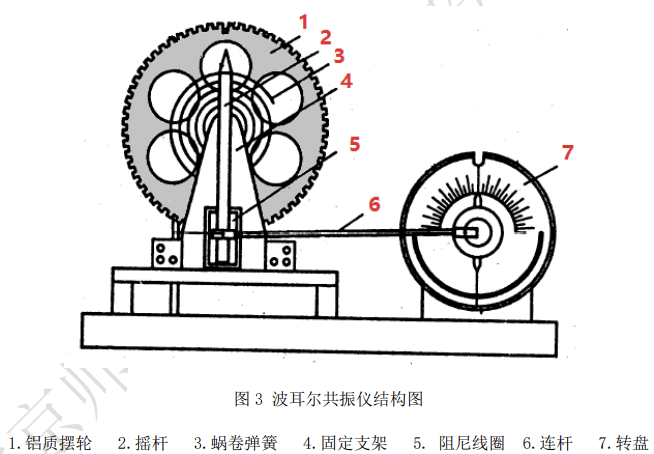
\includegraphics[width=0.5\textwidth]{apparatus.png}
    \caption{波耳共振仪结构图}
    \label{fig:apparatus}
\end{figure}

\subsection{实验步骤}
\subsubsection{衰减法测量振子的固有频率和品质因数}
\begin{enumerate}
    \item 不加驱动,阻尼线圈的电压从8-12V范围取值并固定。
    \item 手动让振子偏离平衡位置,然后释放,记录衰减振动曲线 $\theta(t)$。
    \item 得到数据如下图2所示:
    
\begin{figure}[htbp]
    \centering
    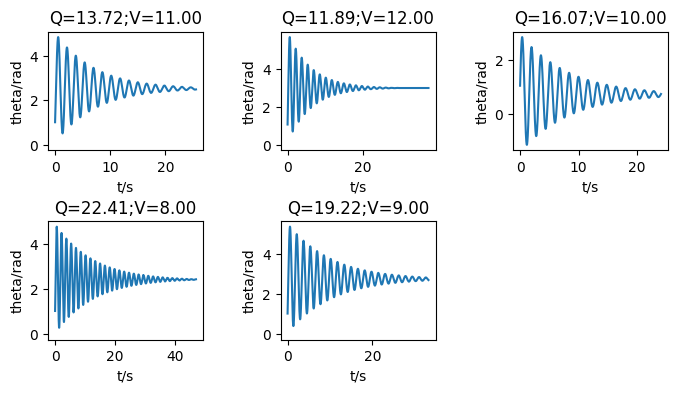
\includegraphics[width=0.7\textwidth]{Q.png}
    \caption{衰减振动曲线}
    \label{fig:Q}
\end{figure}

    \item 用Capstone软件自带的“阻尼正弦” $\theta(t) = Ae^{-Bt} \sin(\omega t + \phi)$ 拟合实验数据。
    \item 根据拟合参数计算 $\omega_0$ 和 $Q$:
    \begin{equation}
    \omega_0 = \sqrt{\omega^2 + B^2}, \quad Q = \frac{\omega_0}{2B}
    \end{equation}
    \item 实验拟合得到\(\omega\)均为3.92rad/s。可见,不同阻尼下的固有频率变化极小,品质因数随阻尼变化较为明显。
    \item 改变线圈电压,重复以上步骤。
\end{enumerate}

\subsubsection{测量电动机驱动信号频率($f$)与驱动圆频率 ($\omega$)之间的关系}
\begin{enumerate}
    \item 设定步进电动机的控制信号,输出1设为直流电压15V,输出2设为方波信号。
    \item 记录摇杆的角度变化曲线,用Capstone软件拟合实验数据,得到驱动频率 $\omega$。
    \item 多次改变电动机转速 $f$,测量相应驱动频率 $\omega$,并进行回归,得到结果如图3,\(r=0.9996\)。
    \begin{figure}[htbp]
        \centering
        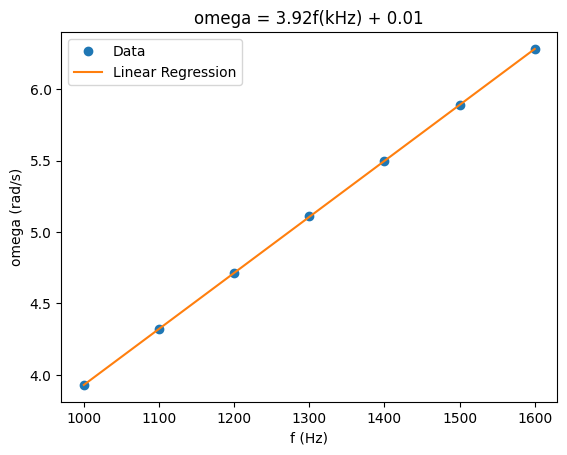
\includegraphics[width=0.6\textwidth]{drive.png}
        \caption{步进电机驱动频率相应}
        \label{fig:drive}
    \end{figure}
    
    \item 根据公式计算 $N = \frac{2\pi f}{\omega}=1600$。
\end{enumerate}

\subsubsection{稳态振动测量}
\begin{enumerate}
    \item 固定阻尼线圈电压为8V和10V,测量幅-频特性和相频特性曲线。
    \item 选择适当测量点,记录振动达到稳定后的数据,如下表所示。
    \begin{table}[H]
    \centering
    \begin{tabular}{lllll}
    \toprule
    \(\bar{\omega}/\omega_0\)&幅值(8V)&幅值(10V)&相位差(8V)&相位差(10V)\\
    \midrule
    -5&0.171&0.128&-0.13&-0.125\\
    -2&0.403&0.29&-0.25&-0.27\\
    -1&0.754&0.534&-0.48&-0.47\\
    -0.5&1.19&0.848&-0.78&-0.81\\
    0.5&1.06&0.74&-2.42&-2.41\\
    1&0.649&0.461&-2.63&-2.716\\
    2&0.346&0.246&-2.919&-2.93\\
    5&0.137&0.095&-3.04&-3.03\\
    \bottomrule
    \end{tabular}
    \end{table}

    \item 改变阻尼线圈电压,重复测量,比较不同 $Q$ 值的频率特性曲线,如下图所示。

\end{enumerate}
\begin{figure}[htbp]
    \centering
    \begin{subfigure}
        \centering
        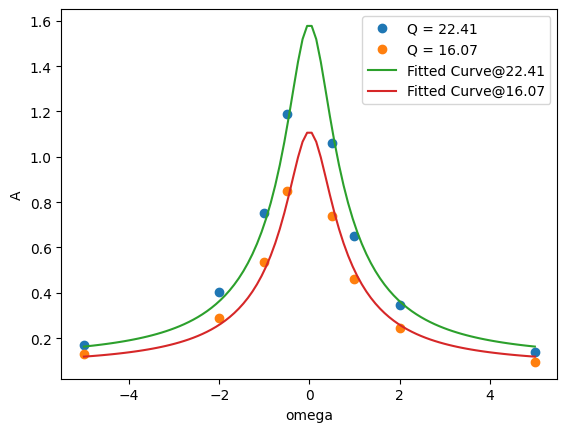
\includegraphics[width=0.6\textwidth]{amplitude.png}
        \caption{不同阻尼下幅频特性曲线}
    \end{subfigure}
    \centering
    \begin{subfigure}
        \centering
        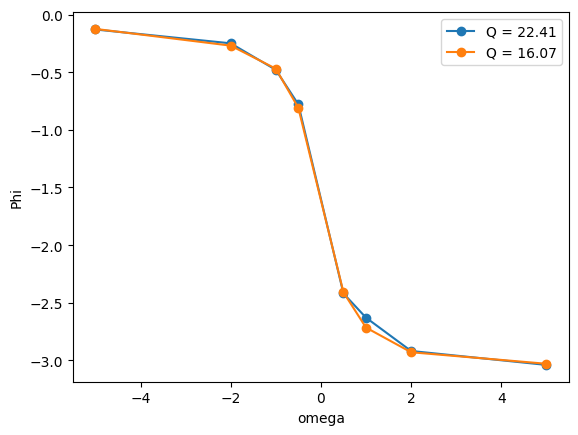
\includegraphics[width=0.6\textwidth]{phase.png}
        \caption{不同阻尼下相频特性曲线}    
    \end{subfigure}
\end{figure}
\newpage
\section{复习思考题解答}

\subsection{振子的品质因数对振子运动特性的影响}
振子的品质因数 \( Q \) 在以下几个方面决定了振子的运动特性:

1. 阻尼大小:品质因数 \( Q \) 越大,阻尼越小。阻尼小意味着系统耗散的能量较少,振子能够维持振动的时间越长。阻尼振动方程为:
   \[
   \frac{d^2 x}{dt^2} + \frac{\omega_0}{Q} \frac{dx}{dt} + \omega_0^2 x = 0
   \]
   其中,无量纲的正数 \( Q \) 表示品质因数。

2. 共振峰的高度和宽度:在共振时,振幅最大,共振峰的高度与品质因数成正比,而宽度与品质因数成反比。即 \( Q \) 越大,共振峰越高且越窄。
   \[
   g = \frac{hQ \omega_0^2}{\sqrt{(\omega^2 - \omega_0^2)^2 + \left(\frac{\omega \omega_0}{Q}\right)^2}}
   \]
   当 \( \omega = \omega_0 \) 时, \( g = Qh \)。

3. 稳态振动的相频特性:相频特性曲线在 \( \omega = \omega_0 \) 时, \( \varphi = -\frac{\pi}{2} \),即驱动力与振子速度同相,能量传递效率最高。 \( Q \) 越大,相位差在共振附近变化越快。
   \[
   \varphi = \cot^{-1} \left[Q \left( \frac{\omega}{\omega_0} - \frac{\omega_0}{\omega} \right)\right]
   \]
   当 \( \omega \rightarrow 0 \) 时, \( \varphi \rightarrow 0 \),当 \( \omega \rightarrow \infty \) 时, \( \varphi \rightarrow -\pi \)。

4. 系统的响应速度:品质因数 \( Q \) 越大,系统对外界驱动的响应越快,达到稳态振动所需的时间越短。

\subsection{实验结果与理论模型的符合及差异分析}
在实验中,我们观察到了以下结果与理论模型的符合与差异:

1. 符合部分:
   - 衰减振动曲线的拟合效果较好,说明摩擦力矩与速度成正比的假设合理。
   - 在共振频率附近,振幅达到最大值,验证了共振现象与理论模型的预期一致。

2. 差异部分:
   - 在频率特性曲线测量中,不同 \( Q \) 值下,频率特性曲线在 \( \omega_0 \) 附近的变化未完全如理论预期,存在实验误差。
   - 实际测量过程中,由于实验装置的非线性因素(如传感器误差、驱动不稳定性等),导致测量值与理论值存在偏差。

\subsection{差异原因分析}
1. 实验装置的非线性因素:实验装置如波耳共振仪的机械结构及电子元件的非线性特性可能导致测量值偏差。

2. 实验误差:在测量过程中,数据采集的精度、实验环境的扰动等都会引入误差。

3. 系统稳定性:在共振频率附近,由于系统对频率变化极其敏感,稍有波动就可能引起较大误差。

通过分析,我们认识到在进行物理实验时,除了理论计算外,还需要充分考虑实验装置的实际特性及各种可能的误差来源,以提高实验数据的准确性和可靠性。


\bibliographystyle{plain}
\bibliography{./template}  %bib文件名

\end{document}
